\documentclass[10pt]{beamer}
\usetheme{Madrid}
\usecolortheme{default}

% Packages
\usepackage[english]{babel}
\usepackage{amsmath, amsthm, amssymb}
\usepackage{graphicx}
\usepackage{xcolor}
\usepackage{tcolorbox}
\tcbuselibrary{theorems,breakable}
\usepackage{booktabs}

% Macros
\newcommand{\R}{\mathbb{R}}
\newcommand{\E}{\mathbb{E}}
\newcommand{\p}{\mathbb{P}}
\newcommand{\Cov}{\text{Cov}}
\newcommand{\Var}{\text{Var}}
\newcommand{\RV}{\text{RV}}
\newcommand{\zp}[1]{\|#1\|}
\DeclareMathOperator*{\argmax}{arg\,max}

% Custom boxes
\newtcolorbox{explanationbox}[1]{
    colback=blue!5!white,
    colframe=blue!75!black,
    title=#1,
    fonttitle=\bfseries,
    fontupper=\small
}

\newtcolorbox{boundbox}[1]{
    colback=green!5!white,
    colframe=green!75!black,
    title=#1,
    fonttitle=\bfseries,
    fontupper=\small
}

\newtcolorbox{rhobox}[1]{
    colback=orange!5!white,
    colframe=orange!75!black,
    title=#1,
    fonttitle=\bfseries,
    fontupper=\small
}

% Title information
\title{Functional Extreme Partial Least Squares}
\subtitle{Unraveling the Intuition and Empirical Validation}
\author{Janis Aiad \quad Simon Elis}
\institute{Master MVA - Statistical Learning with Extreme Values\\ENS Paris Saclay}
\date{}

\begin{document}

% Title slide
\begin{frame}
\titlepage
\end{frame}

% Table of contents
\begin{frame}{Outline}
\tableofcontents
\end{frame}

% First section
\section{Introduction}

% Slide 1: PCA vs PLS
\begin{frame}{PCA vs PLS: The Fundamental Distinction}
\begin{columns}
\column{0.5\textwidth}
\textbf{PCA (Unsupervised)}
\begin{itemize}
    \item Operates solely on $X$
    \item Maximizes \emph{variance}
    \item Ignores relationship with $Y$
    \item May prioritize irrelevant directions
\end{itemize}

\column{0.5\textwidth}
\textbf{PLS (Supervised)}
\begin{itemize}
    \item Uses both $X$ and $Y$
    \item Maximizes \emph{covariance} with $Y$
    \item Finds predictive directions
    \item Directly relevant to prediction
\end{itemize}
\end{columns}

\vspace{0.5cm}
\begin{center}
\textbf{FEPLS = PLS for extremes:} Focus on covariance with $Y$ \emph{in the tail}
\end{center}
\end{frame}

% Theory section
\section{Theory : linear regression only for extremes}

% Slide 2: Model Presentation
\begin{frame}{The FEPLS Model}
\textbf{Problem:} Given $(Y, X)$, find direction $w$ that best explains extreme $Y$ values.

\vspace{0.3cm}
\begin{block}{FEPLS Optimization}
\[
w(y) := \argmax_{\zp{w} = 1} \Cov\big( \langle w, X \rangle, Y \mid Y \ge y\big)
\]
\end{block}

\vspace{0.3cm}
\textbf{Inverse Model Assumption:}
\[
X = g(Y)\beta + \varepsilon, \quad \beta \in H, \quad \zp{\beta} = 1, \quad g(x) \sim x^\kappa
\]

\begin{explanationbox}{What's fixed and what's chosen?}
\begin{itemize}
    \item \textbf{$g$ ($\kappa$):} Real-world relationship (data-generating process)
    \item \textbf{$\varphi$ ($\tau$):} User-chosen test function (tuning parameter)
\end{itemize}
\end{explanationbox}
\end{frame}



\begin{frame}{Example: Concave Function with Asymptotes}

\begin{center}
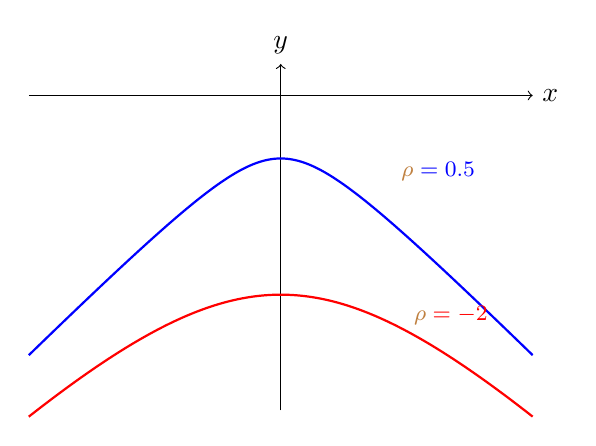
\begin{tikzpicture}[scale=0.8]
    % Axes
    \draw[->] (-4,0) -- (4,0) node[right] {$x$};
    \draw[->] (0,-5) -- (0,0.5) node[above] {$y$};

    % Blue curve (rho = 0.5)
    \draw[domain=-4:4, smooth, thick, blue, samples=100] plot (\x, {-sqrt(1+(\x)*(\x))});
    \node[blue] at (2.5,-1.2) {\footnotesize $\textcolor{brown}{\rho} = 0.5$};

    % Red curve (rho = -2)
    \draw[domain=-4:4, smooth, thick, red, samples=100] plot (\x, {-sqrt(10+(\x)*(\x))});
    \node[red] at (2.7,-3.5) {\footnotesize $\textcolor{brown}{\rho} = -2$};

\end{tikzpicture}
\end{center}

\vspace{0.5cm}
\textbf{Interpretation of the parameter $\textcolor{brown}{\rho}$:} The \textcolor{red}{red} curve ($\textcolor{brown}{\rho} = -2$) has a smaller $\textcolor{brown}{\rho}$ than the \textcolor{blue}{blue} curve ($\textcolor{brown}{\rho} = 0.5$). A more negative $\textcolor{brown}{\rho}$ corresponds to a straighter tail (slower departure from the pure Pareto law).

\end{frame}











% Slide 3: Model Tuning - Parameters
\begin{frame}{Parameter Tuning: What's Estimated, What's Chosen?}
\begin{columns}
\column{0.5\textwidth}
\textbf{Estimated from data:}
\begin{itemize}
    \item $\frac{1}{\textcolor{ForestGreen}{\gamma}}$ exponent  \rightarrow  $ \ \ \ \textcolor{ForestGreen}{\gamma}$ = Tail index of $Y$ (Hill estimator)
    \item $\textcolor{brown}{\rho}$: Second-order parameter (2RV) \rightarrow  $\textcolor{brown}{\rho}$ = Concave curvature of the tail
\end{itemize}


\begin{block}{FEPLS Estimator}
\[
\hat{\beta}_\varphi(y) := \frac{\sum_{i=1}^n X_i Y_i \mathbf{1}_{\{Y_i \geq y\}}}{\left\|\sum_{i=1}^n X_i Y_i \mathbf{1}_{\{Y_i \geq y\}}\right\|}
\]
where $\varphi(x) = x^\tau$ and $g(x) = x^\kappa$ ,  $y = Y_{n-\textcolor{orange}{k}+1,n} \approx U\!\left(\frac{n}{\textcolor{orange}{k}}\right)^{\textcolor{ForestGreen}{\gamma}}$
\end{block}


\vspace{0.3cm}
\textbf{Chosen/Tuned:}
\begin{itemize}
    \item $\tau$: Test function index (tau tuning)
    \item $\textcolor{orange}{k}$: Number of extremes (k tuning)
\end{itemize}

\column{0.5\textwidth}
\begin{rhobox}{Moment Condition}
$0 < 2(\underbrace{\kappa}_{g}+\underbrace{\tau}_{\varphi})\textcolor{ForestGreen}{\gamma} < 1$

Ensures moments exist. Tuning $\tau$:
\begin{itemize}
    \item Large $\tau$: Focus on deepest extremes
    \item Negative $\tau$: Better stability
\end{itemize}
\end{rhobox}
\end{columns}


\vspace{0.3cm}
\textbf{Signal Dominance condition:} $q\kappa\textcolor{ForestGreen}{\gamma} > 1$ (ensures identifiability)
\end{frame}














% Slide 4: Convergence - Choice of k and Bias-Variance
\begin{frame}{Convergence: Choice of $\textcolor{orange}{k}$ and Bias-Variance Tradeoff}
\begin{rhobox}{Optimal Choice of $\textcolor{orange}{k}$}
Balancing bias and variance:
\[
\mathrm{error}(n, \textcolor{orange}{k}) \approx \,(n/\textcolor{orange}{k})^{\textcolor{brown}{\rho}} + \,\textcolor{orange}{k}^{-1/2}
\]
\begin{itemize}
    \item $(n/\textcolor{orange}{k})^{\textcolor{brown}{\rho}}$: Bias (2RV approximation error)
    \item $\textcolor{orange}{k}^{-1/2}$: Variance (statistical noise)
\end{itemize}

Optimal: $\textcolor{orange}{k}_n \sim c\, n^{-2\textcolor{brown}{\rho}/(1-2\textcolor{brown}{\rho})}$ for $\textcolor{brown}{\rho} < 0$
\end{rhobox}

\vspace{0.3cm}
\begin{columns}
\column{0.5\textwidth}
\textbf{Bias-Variance Dilemma:}
\begin{itemize}
    \item Small $\textcolor{orange}{k}$: Low bias, high variance
    \item Large $\textcolor{orange}{k}$: Lower variance, higher bias
\end{itemize}

\column{0.5\textwidth}
\textbf{2RV Interpretation:}
$\textcolor{brown}{\rho}$ quantifies how fast the tail deviates from pure Pareto. More negative $\textcolor{brown}{\rho}$ = straighter tail = easier estimation.
\end{columns}
\end{frame}

% Slide 5: Convergence Scaling Law
\begin{frame}{Convergence Rate: Scaling Law}
\begin{theorem}[FEPLS Consistency]
Under all the conditions, the FEPLS estimator satisfies:
\[
\|\hat{\beta}_\varphi(Y_{n-\textcolor{orange}{k}+1,n}) - \beta\| = O_P(\delta_{n,\textcolor{orange}{k}})
\]
where
\[
\delta_{n,\textcolor{orange}{k}} \sim n^{(1/q-\textcolor{ForestGreen}{\gamma}\kappa)/(1-2\textcolor{brown}{\rho})}
\]
\end{theorem}

\vspace{0.3cm}
\begin{block}{Key Insights}
\begin{itemize}
    \item Convergence rate depends on $\textcolor{ForestGreen}{\gamma}$, $\kappa$, $q$, and $\textcolor{brown}{\rho}$
    \item For $\textcolor{brown}{\rho} < 0$: Explicit rate $O(n^{(1/q-\textcolor{ForestGreen}{\gamma}\kappa)/(1-2\textcolor{brown}{\rho})})$
    \item Optimal $\textcolor{orange}{k}$: $\textcolor{orange}{k}_n \sim c\, n^{-2\textcolor{brown}{\rho}/(1-2\textcolor{brown}{\rho})}$ balances bias and variance
\end{itemize}
\end{block}
\end{frame}

% Practice section
\section{Practice}

% Slide 6: Empirical Results - Overview
\begin{frame}{Empirical Results: Overview}

We done a lot of simulations and experiments (35 coding hours) to produce those results !

\vspace{0.18cm}

\textbf{Two Settings:}
\begin{enumerate}
    \item \textbf{Low-frequency (daily):} Hungarian stock market (Stooq data)
    \begin{itemize}
        \item 4IG paired with multiple stocks (3500 pairs)
        \item Good Hill estimation: $\textcolor{ForestGreen}{\gamma} \in [0.2, 0.4]$ (very consistent)
        \item Limited samples: $\textcolor{orange}{k} < 10$
    \end{itemize}
    
    \item \textbf{High-frequency (5-min):} AAPL intraday data
    \begin{itemize}
        \item 5-minute windows
        \item Large sample: $\textcolor{orange}{k}$ up to 800
        \item Microstructure effects challenge Hill estimation
    \end{itemize}
\end{enumerate}
\end{frame}

% Slide 7: Low-Frequency Results
\begin{frame}{Low-Frequency Results: Hungarian Stock Market}
\begin{columns}
\column{0.5\textwidth}
\textbf{Key Findings:}
\begin{itemize}
    \item Hill estimator: $\textcolor{ForestGreen}{\gamma} \in [0.2, 0.4]$ (very consistent)
    \item Limited extremes: $\textcolor{orange}{k} < 10$
    \item $\tau$ dependency crucial for noisy, small-sample regime
\end{itemize}

\vspace{0.3cm}
\textbf{Stock Groups:}
\begin{itemize}
    \item \textcolor{green}{Sensitive:} End-of-day volatility drives next day's max
    \item \textcolor{red}{Insensitive:} No clear relationship
\end{itemize}

\column{0.5\textwidth}
\begin{center}
\includegraphics[width=\textwidth]{figures/4ig_akko_hill_qq_tail.png}
\end{center}
\end{columns}

\vspace{0.3cm}
\textbf{Interpretation:} Cross-asset dependencies and volatility spillover mechanisms
\end{frame}

% Slide 8: High-Frequency Results
\begin{frame}{High-Frequency Results: AAPL 5-Minute Data}
\begin{columns}
\column{0.5\textwidth}
\textbf{Setup:}
\begin{itemize}
    \item $X$: 5-minute return window
    \item $Y$: Max of next 5-minute window
        \item Large sample: $\textcolor{orange}{k}$ from 0 to 800
\end{itemize}

\vspace{0.3cm}
\textbf{Challenges:}
\begin{itemize}
    \item Hill estimator poorly estimated (microstructure)
    \item Q-Q plot shows poor fit
\end{itemize}

\column{0.5\textwidth}
\begin{center}
\includegraphics[width=\textwidth]{figures/AAPL_5min_d10_k5_tau_-0.5.png}
\end{center}
\end{columns}

\vspace{0.3cm}
\textbf{Key Finding:} Clear increasing relationship $\Rightarrow$ \textcolor{blue}{\textbf{Mid-frequency is trend-driven!}}
\end{frame}

% Slide 9: Hill-QQ-Tail Plots Grid
\begin{frame}{Diagnostic Plots: Hill, Q-Q, and Tail Analysis}
\begin{center}
\includegraphics[width=0.9\textwidth]{figures/4ig_bif_hill_qq_tail.png}
\end{center}

\vspace{0.2cm}
\textbf{Multiple stock pairs show:}
\begin{itemize}
    \item Consistent Hill estimates ($\textcolor{ForestGreen}{\gamma} \in [0.2, 0.4]$)
    \item Good Q-Q plot fit for low-frequency data
    \item Clear tail behavior suitable for FEPLS
\end{itemize}
\end{frame}

% Slide 10: Beta Comparison and Conclusions
\begin{frame}{Beta Stability and Conclusions}
\begin{columns}
\column{0.5\textwidth}
\textbf{Beta Comparison:}
\begin{itemize}
    \item Stability across $\tau$ values
    \item Sensitivity analysis for test function
    \item Identifies robust directions
\end{itemize}

\vspace{0.3cm}
\textbf{Main Conclusions:}
\begin{enumerate}
    \item FEPLS works well for heavy-tailed data
    \item $\tau$ tuning crucial in small-sample regime
    \item Clear patterns: trend-driven (HF) vs volatility-driven (LF)
\end{enumerate}

\column{0.5\textwidth}
\begin{center}
\includegraphics[width=\textwidth]{figures/4ig_akko_tau_-2.0_-0.5.png}
\end{center}
\end{columns}

\vspace{0.3cm}
\textbf{Practical Impact:} Identifies predictive features for extreme events in financial markets
\end{frame}

\end{document}
